\documentclass[12pt,a4paper]{scrartcl}\usepackage[]{graphicx}\usepackage[]{color}
%% maxwidth is the original width if it is less than linewidth
%% otherwise use linewidth (to make sure the graphics do not exceed the margin)
\makeatletter
\def\maxwidth{ %
  \ifdim\Gin@nat@width>\linewidth
    \linewidth
  \else
    \Gin@nat@width
  \fi
}
\makeatother

\definecolor{fgcolor}{rgb}{0.345, 0.345, 0.345}
\newcommand{\hlnum}[1]{\textcolor[rgb]{0.686,0.059,0.569}{#1}}%
\newcommand{\hlstr}[1]{\textcolor[rgb]{0.192,0.494,0.8}{#1}}%
\newcommand{\hlcom}[1]{\textcolor[rgb]{0.678,0.584,0.686}{\textit{#1}}}%
\newcommand{\hlopt}[1]{\textcolor[rgb]{0,0,0}{#1}}%
\newcommand{\hlstd}[1]{\textcolor[rgb]{0.345,0.345,0.345}{#1}}%
\newcommand{\hlkwa}[1]{\textcolor[rgb]{0.161,0.373,0.58}{\textbf{#1}}}%
\newcommand{\hlkwb}[1]{\textcolor[rgb]{0.69,0.353,0.396}{#1}}%
\newcommand{\hlkwc}[1]{\textcolor[rgb]{0.333,0.667,0.333}{#1}}%
\newcommand{\hlkwd}[1]{\textcolor[rgb]{0.737,0.353,0.396}{\textbf{#1}}}%
\let\hlipl\hlkwb

\usepackage{framed}
\makeatletter
\newenvironment{kframe}{%
 \def\at@end@of@kframe{}%
 \ifinner\ifhmode%
  \def\at@end@of@kframe{\end{minipage}}%
  \begin{minipage}{\columnwidth}%
 \fi\fi%
 \def\FrameCommand##1{\hskip\@totalleftmargin \hskip-\fboxsep
 \colorbox{shadecolor}{##1}\hskip-\fboxsep
     % There is no \\@totalrightmargin, so:
     \hskip-\linewidth \hskip-\@totalleftmargin \hskip\columnwidth}%
 \MakeFramed {\advance\hsize-\width
   \@totalleftmargin\z@ \linewidth\hsize
   \@setminipage}}%
 {\par\unskip\endMakeFramed%
 \at@end@of@kframe}
\makeatother

\definecolor{shadecolor}{rgb}{.97, .97, .97}
\definecolor{messagecolor}{rgb}{0, 0, 0}
\definecolor{warningcolor}{rgb}{1, 0, 1}
\definecolor{errorcolor}{rgb}{1, 0, 0}
\newenvironment{knitrout}{}{} % an empty environment to be redefined in TeX

\usepackage{alltt}
\usepackage[utf8]{inputenc}
\usepackage{amsmath}
\usepackage{graphicx}
\usepackage{tikz}
%\usepackage{silence}
\usepackage{mdframed}
%\WarningFilter{mdframed}{You got a bad break}
\usepackage[colorinlistoftodos]{todonotes}
\usepackage{listings}
\usepackage{color}
\colorlet{exampcol}{blue!10}
\usepackage{multicol}
\usepackage{booktabs}

\usepackage[noanswer]{exercise}%[noanswer]

\usepackage[autostyle, english = american]{csquotes}
\MakeOuterQuote{"}

\usepackage{hyperref}
\hypersetup{
    colorlinks,
    citecolor=black,
    filecolor=black,
    linkcolor=blue,
    urlcolor=black
}

\title{Exercises for linear mixed effect models, part 3}
\date{\today}
\author{Timoth\'ee Bonnet}
\IfFileExists{upquote.sty}{\usepackage{upquote}}{}
\begin{document}



\maketitle

\tableofcontents
\ListOfExerciseInToc
\ExerciseLevelInToc{subsubsection}

\clearpage



\section{Random interactions}

\subsection{Random slopes}



\begin{Exercise}[difficulty=1, title={Random slopes and unbalanced data}]
Load the dataset \texttt{hares.csv}. It contains (fake) measurements of snowshoe hare color (darkness) and their detectability against the background where they live. Measurements were taken in 50 different locations. We want to know whether darkness has an effect on detectability. 
\begin{enumerate}
  \item Fit a simple linear model of detectability on darkness. What is the effect?
  \item Add a random intercept to the previous model. Does it change the result quantitatively?
  \item Add a random slope. What do you see now?
\end{enumerate}
\end{Exercise}
\begin{Answer}
\begin{knitrout}
\definecolor{shadecolor}{rgb}{0.969, 0.969, 0.969}\color{fgcolor}\begin{kframe}
\begin{alltt}
\hlstd{dat} \hlkwb{<-} \hlkwd{read.csv}\hlstd{(}\hlstr{"hares.csv"}\hlstd{)}
\hlkwd{summary}\hlstd{(}\hlkwd{lm}\hlstd{(detectability} \hlopt{~} \hlnum{1} \hlopt{+} \hlstd{darkness,} \hlkwc{data} \hlstd{= dat) )}
\hlkwd{summary}\hlstd{(}\hlkwd{lmer}\hlstd{(detectability} \hlopt{~} \hlnum{1} \hlopt{+} \hlstd{darkness} \hlopt{+} \hlstd{(}\hlnum{1}\hlopt{|}\hlstd{location),} \hlkwc{data} \hlstd{= dat) )}
\hlkwd{summary}\hlstd{(}\hlkwd{lmer}\hlstd{(detectability} \hlopt{~} \hlnum{1} \hlopt{+} \hlstd{darkness} \hlopt{+} \hlstd{(}\hlnum{1}\hlopt{+}\hlstd{darkness}\hlopt{|}\hlstd{location),} \hlkwc{data} \hlstd{= dat) )}
\end{alltt}
\end{kframe}
\end{knitrout}
The direction of the slope changes when you add a random slope (but not when you add a random intercept).
\end{Answer}

\begin{Exercise}[difficulty=2, title={Visualize random slopes}]
Visualize the effect from the random slope model, that is, plot the relationship detectability over darkness for every location. Add the overall relationship (for instance extracted from a simple linear regression). You can use the functions \texttt{ranef()} and \texttt{fixef()}. Why did the fixed effect of darkness changed so much when you added the random slope? 
\end{Exercise}
\begin{Answer}
\begin{knitrout}
\definecolor{shadecolor}{rgb}{0.969, 0.969, 0.969}\color{fgcolor}\begin{kframe}
\begin{alltt}
\hlstd{mhar} \hlkwb{<-} \hlkwd{lmer}\hlstd{(detectability} \hlopt{~} \hlnum{1} \hlopt{+} \hlstd{darkness} \hlopt{+} \hlstd{(}\hlnum{1}\hlopt{+}\hlstd{darkness}\hlopt{|}\hlstd{location),} \hlkwc{data} \hlstd{= dat)}
\end{alltt}


{\ttfamily\noindent\bfseries\color{errorcolor}{\#\# Error: 'data' not found, and some variables missing from formula environment}}\begin{alltt}
\hlstd{rhar} \hlkwb{<-} \hlkwd{ranef}\hlstd{(mhar)}\hlopt{$}\hlstd{location}
\end{alltt}


{\ttfamily\noindent\bfseries\color{errorcolor}{\#\# Error in ranef(mhar): object 'mhar' not found}}\begin{alltt}
\hlstd{fhar} \hlkwb{<-} \hlkwd{fixef}\hlstd{(mhar)}
\end{alltt}


{\ttfamily\noindent\bfseries\color{errorcolor}{\#\# Error in fixef(mhar): object 'mhar' not found}}\begin{alltt}
\hlstd{dark}\hlkwb{<-} \hlkwd{seq}\hlstd{(}\hlkwc{from}\hlstd{=}\hlkwd{min}\hlstd{(dat}\hlopt{$}\hlstd{darkness),} \hlkwc{to}\hlstd{=}\hlkwd{max}\hlstd{(dat}\hlopt{$}\hlstd{darkness),} \hlkwc{length.out} \hlstd{=} \hlnum{100}\hlstd{)}
\end{alltt}


{\ttfamily\noindent\bfseries\color{errorcolor}{\#\# Error in seq(from = min(dat\$darkness), to = max(dat\$darkness), length.out = 100): object 'dat' not found}}\begin{alltt}
\hlcom{#first we plot the MEDIAN relationship, that is, the slope to the }
\hlcom{# hypothetical location with random effects of zero}

\hlkwd{plot}\hlstd{(}\hlkwc{x}\hlstd{=dark,} \hlkwc{y}\hlstd{=fhar[}\hlnum{1}\hlstd{]}\hlopt{+}\hlstd{dark}\hlopt{*}\hlstd{fhar[}\hlnum{2}\hlstd{],} \hlkwc{ylim}\hlstd{=}\hlkwd{c}\hlstd{(}\hlnum{0}\hlstd{,}\hlnum{4}\hlstd{),} \hlkwc{type}\hlstd{=}\hlstr{"l"}\hlstd{,}
     \hlkwc{lwd}\hlstd{=}\hlnum{5}\hlstd{,} \hlkwc{lty}\hlstd{=}\hlnum{2}\hlstd{,} \hlkwc{main}\hlstd{=}\hlstr{"Mean effect (dotted),
     Median effect (dashed) and location slopes"}\hlstd{)}
\end{alltt}


{\ttfamily\noindent\bfseries\color{errorcolor}{\#\# Error in plot(x = dark, y = fhar[1] + dark * fhar[2], ylim = c(0, 4), : object 'dark' not found}}\begin{alltt}
\hlcom{#then we plot slopes for each locations}
\hlstd{cls} \hlkwb{<-} \hlkwd{rainbow}\hlstd{(}\hlkwc{n} \hlstd{=} \hlkwd{nrow}\hlstd{(rhar))}
\end{alltt}


{\ttfamily\noindent\bfseries\color{errorcolor}{\#\# Error in nrow(rhar): object 'rhar' not found}}\begin{alltt}
\hlkwa{for}\hlstd{(i} \hlkwa{in} \hlnum{1}\hlopt{:}\hlkwd{nrow}\hlstd{(rhar))}
\hlstd{\{}
  \hlkwd{lines}\hlstd{(}\hlkwc{x}\hlstd{=dark,} \hlkwc{y}\hlstd{=(fhar[}\hlnum{1}\hlstd{]}\hlopt{+}\hlstd{rhar[i,}\hlnum{1}\hlstd{])}\hlopt{+}\hlcom{#intercept for location i}
          \hlstd{dark}\hlopt{*}\hlstd{(fhar[}\hlnum{2}\hlstd{]}\hlopt{+}\hlstd{rhar[i,}\hlnum{2}\hlstd{]),}\hlcom{# slope for location i}
    \hlkwc{col}\hlstd{=cls[i])}
\hlstd{\}}
\end{alltt}


{\ttfamily\noindent\bfseries\color{errorcolor}{\#\# Error in nrow(rhar): object 'rhar' not found}}\begin{alltt}
\hlstd{m0har} \hlkwb{<-} \hlkwd{lm}\hlstd{(detectability} \hlopt{~} \hlnum{1} \hlopt{+} \hlstd{darkness,} \hlkwc{data} \hlstd{= dat)}
\end{alltt}


{\ttfamily\noindent\bfseries\color{errorcolor}{\#\# Error in is.data.frame(data): object 'dat' not found}}\begin{alltt}
\hlkwd{abline}\hlstd{(m0har,} \hlkwc{lwd}\hlstd{=}\hlnum{5}\hlstd{,} \hlkwc{lty}\hlstd{=}\hlnum{3}\hlstd{)}
\end{alltt}


{\ttfamily\noindent\bfseries\color{errorcolor}{\#\# Error in abline(m0har, lwd = 5, lty = 3): object 'm0har' not found}}\begin{alltt}
\hlkwd{legend}\hlstd{(}\hlkwc{x} \hlstd{=} \hlstr{"topleft"}\hlstd{,} \hlkwc{legend} \hlstd{=} \hlkwd{c}\hlstd{(}\hlstr{"Simple regression"}\hlstd{,} \hlstr{"Random slope"}\hlstd{),}
       \hlkwc{lwd}\hlstd{=}\hlnum{5}\hlstd{,} \hlkwc{lty} \hlstd{=} \hlkwd{c}\hlstd{(}\hlnum{3}\hlstd{,}\hlnum{2}\hlstd{))}
\end{alltt}


{\ttfamily\noindent\bfseries\color{errorcolor}{\#\# Error in strwidth(legend, units = "{}user"{}, cex = cex, font = text.font): plot.new has not been called yet}}\end{kframe}
\end{knitrout}

The problem with the simple regression comes from the imbalance in the data! One location has a positive relationship, while the 49 others have a negative relationship. The simple regression is also positive. Why does one location have so much weight?
Let's look at sample sizes per location:
\begin{knitrout}
\definecolor{shadecolor}{rgb}{0.969, 0.969, 0.969}\color{fgcolor}\begin{kframe}
\begin{alltt}
\hlkwd{table}\hlstd{(dat}\hlopt{$}\hlstd{location)}
\end{alltt}


{\ttfamily\noindent\bfseries\color{errorcolor}{\#\# Error in table(dat\$location): object 'dat' not found}}\end{kframe}
\end{knitrout}

510 observations come from location 50! That is why it weights so much in the simple regression. In contrast the random slope can tell the mean effect from the mediam slope.
\end{Answer}



\begin{Exercise}[difficulty=2, title={Does natural selection vary?}]
Load the dataset \texttt{AllM.txt}. It contains true data from the long term monitoring of a wild animal population. We are interested in quantifying natural selection on Weight. To simplify let's assume natural selection is the slope of \texttt{fitnessR} on \texttt{Weight}. 
\begin{enumerate}
  \item Fit a linear regression of fitnessR on Weight. Include \texttt{Age} as a predictor Is there evidence for selection?
  \item Change your model to a mixed model with year as a random intercept. Do you think fitnessR varies a lot among years?
  \item Now add a random slope on weight. How much variation is there in selection?
  \item Make a graph to visualize selection on different years (the function \texttt{ranef()} extract random effects) (you can make the graph for adults, for juveniles, or both).
  \item Looking at the estimated variance for the intercept and for Weight, which one looks more important? Is that your impression graphically? Why?
  \item Bonus: test for the statistical significance of the variation in selection (you can use \texttt{anova()} to compare two models).
\end{enumerate}
\end{Exercise}
\begin{Answer}
Careful here! The dataset is a text file, not a csv file! You need to load the data using \texttt(read.table()) with the argument \texttt{header=TRUE}!
\begin{knitrout}
\definecolor{shadecolor}{rgb}{0.969, 0.969, 0.969}\color{fgcolor}\begin{kframe}
\begin{alltt}
\hlkwd{library}\hlstd{(lme4)}
\hlstd{allm} \hlkwb{<-} \hlkwd{read.table}\hlstd{(}\hlstr{"AllM.txt"}\hlstd{,} \hlkwc{header} \hlstd{=} \hlnum{TRUE}\hlstd{)}
\end{alltt}
\end{kframe}
\end{knitrout}

1. Simple linear regression
\begin{knitrout}
\definecolor{shadecolor}{rgb}{0.969, 0.969, 0.969}\color{fgcolor}\begin{kframe}
\begin{alltt}
\hlstd{mlr} \hlkwb{<-} \hlkwd{lm}\hlstd{(fitnessR} \hlopt{~} \hlnum{1} \hlopt{+} \hlstd{Age} \hlopt{+} \hlstd{Weight,} \hlkwc{data} \hlstd{= allm)}
\hlkwd{summary}\hlstd{(mlr)}
\end{alltt}
\begin{verbatim}
## 
## Call:
## lm(formula = fitnessR ~ 1 + Age + Weight, data = allm)
## 
## Residuals:
##    Min     1Q Median     3Q    Max 
## -4.243 -1.258 -0.602  1.058 11.958 
## 
## Coefficients:
##             Estimate Std. Error t value Pr(>|t|)    
## (Intercept)  0.35759    0.34410    1.04      0.3    
## AgeJ        -1.31987    0.15564   -8.48   <2e-16 ***
## Weight       0.06937    0.00808    8.59   <2e-16 ***
## ---
## Signif. codes:  0 '***' 0.001 '**' 0.01 '*' 0.05 '.' 0.1 ' ' 1
## 
## Residual standard error: 2.31 on 2906 degrees of freedom
##   (114 observations deleted due to missingness)
## Multiple R-squared:  0.227,	Adjusted R-squared:  0.227 
## F-statistic:  428 on 2 and 2906 DF,  p-value: <2e-16
\end{verbatim}
\end{kframe}
\end{knitrout}
It looks like there is selection for heavier individuals.\\

2. Random intercept
\begin{knitrout}
\definecolor{shadecolor}{rgb}{0.969, 0.969, 0.969}\color{fgcolor}\begin{kframe}
\begin{alltt}
\hlstd{mri} \hlkwb{<-} \hlkwd{lmer}\hlstd{(fitnessR} \hlopt{~} \hlnum{1}\hlopt{+} \hlstd{Age}  \hlopt{+} \hlstd{Weight} \hlopt{+} \hlstd{(}\hlnum{1}\hlopt{|}\hlstd{Year),} \hlkwc{data} \hlstd{= allm)}
\hlkwd{summary}\hlstd{(mri)}
\end{alltt}
\begin{verbatim}
## Linear mixed model fit by REML ['lmerMod']
## Formula: fitnessR ~ 1 + Age + Weight + (1 | Year)
##    Data: allm
## 
## REML criterion at convergence: 12956
## 
## Scaled residuals: 
##    Min     1Q Median     3Q    Max 
## -2.161 -0.585 -0.238  0.442  5.062 
## 
## Random effects:
##  Groups   Name        Variance Std.Dev.
##  Year     (Intercept) 0.595    0.771   
##  Residual             4.966    2.228   
## Number of obs: 2909, groups:  Year, 8
## 
## Fixed effects:
##             Estimate Std. Error t value
## (Intercept)  0.47454    0.43158     1.1
## AgeJ        -1.57284    0.15241   -10.3
## Weight       0.06283    0.00786     8.0
## 
## Correlation of Fixed Effects:
##        (Intr) AgeJ  
## AgeJ   -0.676       
## Weight -0.763  0.830
\end{verbatim}
\end{kframe}
\end{knitrout}
Some years have much higher or much lower fitness on average.\\

3.Random slope
\begin{knitrout}
\definecolor{shadecolor}{rgb}{0.969, 0.969, 0.969}\color{fgcolor}\begin{kframe}
\begin{alltt}
\hlstd{mrs} \hlkwb{<-} \hlkwd{lmer}\hlstd{(fitnessR} \hlopt{~} \hlnum{1}\hlopt{+} \hlstd{Age}  \hlopt{+} \hlstd{Weight}  \hlopt{+} \hlstd{(}\hlnum{1}\hlopt{+} \hlstd{Weight}\hlopt{|}\hlstd{Year),} \hlkwc{data} \hlstd{= allm)}
\hlkwd{summary}\hlstd{(mrs)}
\end{alltt}
\begin{verbatim}
## Linear mixed model fit by REML ['lmerMod']
## Formula: fitnessR ~ 1 + Age + Weight + (1 + Weight | Year)
##    Data: allm
## 
## REML criterion at convergence: 12872
## 
## Scaled residuals: 
##    Min     1Q Median     3Q    Max 
## -2.478 -0.570 -0.205  0.432  5.174 
## 
## Random effects:
##  Groups   Name        Variance Std.Dev. Corr 
##  Year     (Intercept) 1.8465   1.359         
##           Weight      0.0026   0.051    -0.94
##  Residual             4.8037   2.192         
## Number of obs: 2909, groups:  Year, 8
## 
## Fixed effects:
##             Estimate Std. Error t value
## (Intercept)   1.1515     0.5918    1.95
## AgeJ         -1.5632     0.1510  -10.35
## Weight        0.0444     0.0198    2.24
## 
## Correlation of Fixed Effects:
##        (Intr) AgeJ  
## AgeJ   -0.490       
## Weight -0.932  0.328
\end{verbatim}
\end{kframe}
\end{knitrout}
Selection may fluctuate (the variance component for the slope of Weight is not null), but it looks small and it is very correlated to the random intercept. So it is difficult to tell.\\

4.Visualize
\begin{knitrout}
\definecolor{shadecolor}{rgb}{0.969, 0.969, 0.969}\color{fgcolor}\begin{kframe}
\begin{alltt}
\hlstd{wgt} \hlkwb{<-} \hlkwd{seq}\hlstd{(}\hlnum{10}\hlstd{,}\hlnum{50}\hlstd{,} \hlkwc{by}\hlstd{=}\hlnum{0.1}\hlstd{)}
\hlkwd{fixef}\hlstd{(mrs)}
\end{alltt}
\begin{verbatim}
## (Intercept)        AgeJ      Weight 
##     1.15147    -1.56323     0.04439
\end{verbatim}
\begin{alltt}
\hlkwd{plot}\hlstd{(}\hlkwc{x}\hlstd{=wgt,} \hlkwc{y}\hlstd{=}\hlkwd{fixef}\hlstd{(mrs)[}\hlnum{1}\hlstd{]} \hlopt{+} \hlkwd{fixef}\hlstd{(mrs)[}\hlnum{3}\hlstd{]}\hlopt{*} \hlstd{wgt,} \hlkwc{ylim} \hlstd{=} \hlkwd{c}\hlstd{(}\hlnum{0}\hlstd{,}\hlnum{5}\hlstd{),}
     \hlkwc{xlab}\hlstd{=}\hlstr{"Weight"}\hlstd{,} \hlkwc{ylab}\hlstd{=}\hlstr{"Fitness"}\hlstd{)}
\hlstd{rde} \hlkwb{<-} \hlkwd{ranef}\hlstd{(mrs)}\hlopt{$}\hlstd{Year}
\hlkwa{for} \hlstd{(i} \hlkwa{in} \hlnum{1}\hlopt{:}\hlkwd{nrow}\hlstd{(rde))}
\hlstd{\{}
  \hlkwd{lines}\hlstd{(}\hlkwc{x}\hlstd{=wgt,} \hlkwc{y}\hlstd{=}\hlkwd{fixef}\hlstd{(mrs)[}\hlnum{1}\hlstd{]}\hlopt{+}  \hlstd{rde[i,}\hlnum{1}\hlstd{]} \hlopt{+} \hlstd{(}\hlkwd{fixef}\hlstd{(mrs)[}\hlnum{3}\hlstd{]}\hlopt{+}\hlstd{rde[i,}\hlnum{2}\hlstd{])}\hlopt{*} \hlstd{wgt)}
\hlstd{\}}
\end{alltt}
\end{kframe}
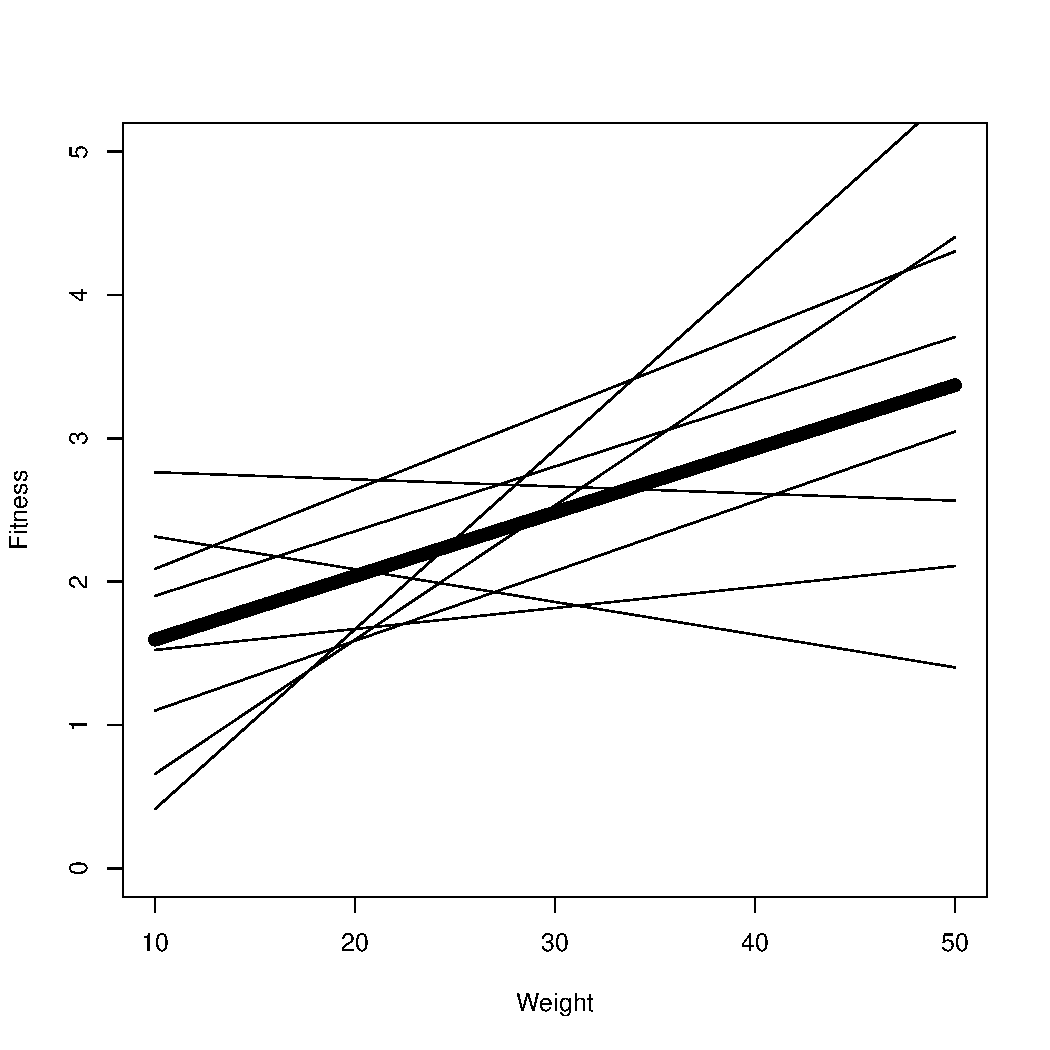
\includegraphics[width=\maxwidth]{figure/unnamed-chunk-10-1} 

\end{knitrout}

5. Statistical test
\begin{knitrout}
\definecolor{shadecolor}{rgb}{0.969, 0.969, 0.969}\color{fgcolor}\begin{kframe}
\begin{alltt}
\hlkwd{anova}\hlstd{(mri,mrs)}
\end{alltt}


{\ttfamily\noindent\itshape\color{messagecolor}{\#\# refitting model(s) with ML (instead of REML)}}\begin{verbatim}
## Data: allm
## Models:
## mri: fitnessR ~ 1 + Age + Weight + (1 | Year)
## mrs: fitnessR ~ 1 + Age + Weight + (1 + Weight | Year)
##     Df   AIC   BIC logLik deviance Chisq Chi Df Pr(>Chisq)    
## mri  5 12954 12984  -6472    12944                            
## mrs  7 12877 12918  -6431    12863  81.2      2     <2e-16 ***
## ---
## Signif. codes:  0 '***' 0.001 '**' 0.01 '*' 0.05 '.' 0.1 ' ' 1
\end{verbatim}
\end{kframe}
\end{knitrout}
You can compare the random intercept only model to the random intercept and random slope model to see if adding the latter improves the fit. The p-value is approximate only, but that doesn't matter because it is tiny anyways. 

\end{Answer}

\subsection{Random factor interaction}












\begin{Exercise}[difficulty=1, title={Random interaction with a factor}]
Load the file \texttt{interfactor.csv} and fit two random interaction modelw of y as a function of treat, using both the reaction norm and the character state approach. How do the estimate differ?
Use the functions \texttt{AIC()}, \texttt{fitted()} and \texttt{resid()} to compare the fit of the two models? What can you conclude?
\end{Exercise}
\begin{Answer}
\begin{knitrout}
\definecolor{shadecolor}{rgb}{0.969, 0.969, 0.969}\color{fgcolor}\begin{kframe}
\begin{alltt}
\hlstd{dat} \hlkwb{<-} \hlkwd{read.csv}\hlstd{(}\hlstr{"interfactor.csv"}\hlstd{)}
\hlkwd{library}\hlstd{(lme4)}
\hlkwd{summary}\hlstd{(mf1} \hlkwb{<-} \hlkwd{lmer}\hlstd{(y} \hlopt{~} \hlnum{1} \hlopt{+} \hlstd{treat} \hlopt{+} \hlstd{(}\hlnum{1}\hlopt{+}\hlstd{treat}\hlopt{|}\hlstd{id),} \hlkwc{data} \hlstd{= dat))}
\end{alltt}
\begin{verbatim}
## Linear mixed model fit by REML ['lmerMod']
## Formula: y ~ 1 + treat + (1 + treat | id)
##    Data: dat
## 
## REML criterion at convergence: -2335
## 
## Scaled residuals: 
##     Min      1Q  Median      3Q     Max 
## -2.4730 -0.6422 -0.0409  0.6072  2.4375 
## 
## Random effects:
##  Groups   Name           Variance Std.Dev. Corr
##  id       (Intercept)    0.1740   0.417        
##           treattreatment 0.0606   0.246    0.45
##  Residual                0.0001   0.010        
## Number of obs: 500, groups:  id, 50
## 
## Fixed effects:
##                Estimate Std. Error t value
## (Intercept)      3.0734     0.0590    52.1
## treattreatment   0.4525     0.0348    13.0
## 
## Correlation of Fixed Effects:
##             (Intr)
## treattrtmnt 0.451
\end{verbatim}
\end{kframe}
\end{knitrout}

\begin{knitrout}
\definecolor{shadecolor}{rgb}{0.969, 0.969, 0.969}\color{fgcolor}\begin{kframe}
\begin{alltt}
\hlkwd{summary}\hlstd{(mf2} \hlkwb{<-} \hlkwd{lmer}\hlstd{(y} \hlopt{~} \hlnum{1} \hlopt{+} \hlstd{treat} \hlopt{+} \hlstd{(}\hlnum{0}\hlopt{+}\hlstd{treat}\hlopt{|}\hlstd{id),} \hlkwc{data} \hlstd{= dat))}
\end{alltt}
\begin{verbatim}
## Linear mixed model fit by REML ['lmerMod']
## Formula: y ~ 1 + treat + (0 + treat | id)
##    Data: dat
## 
## REML criterion at convergence: -2335
## 
## Scaled residuals: 
##     Min      1Q  Median      3Q     Max 
## -2.4730 -0.6422 -0.0409  0.6072  2.4375 
## 
## Random effects:
##  Groups   Name           Variance Std.Dev. Corr
##  id       treatcontrol   0.1740   0.417        
##           treattreatment 0.3272   0.572    0.92
##  Residual                0.0001   0.010        
## Number of obs: 500, groups:  id, 50
## 
## Fixed effects:
##                Estimate Std. Error t value
## (Intercept)      3.0734     0.0590    52.1
## treattreatment   0.4525     0.0348    13.0
## 
## Correlation of Fixed Effects:
##             (Intr)
## treattrtmnt 0.451
\end{verbatim}
\begin{alltt}
\hlkwd{plot}\hlstd{(}\hlkwd{fitted}\hlstd{(mf1),} \hlkwd{fitted}\hlstd{(mf2))}
\end{alltt}
\end{kframe}
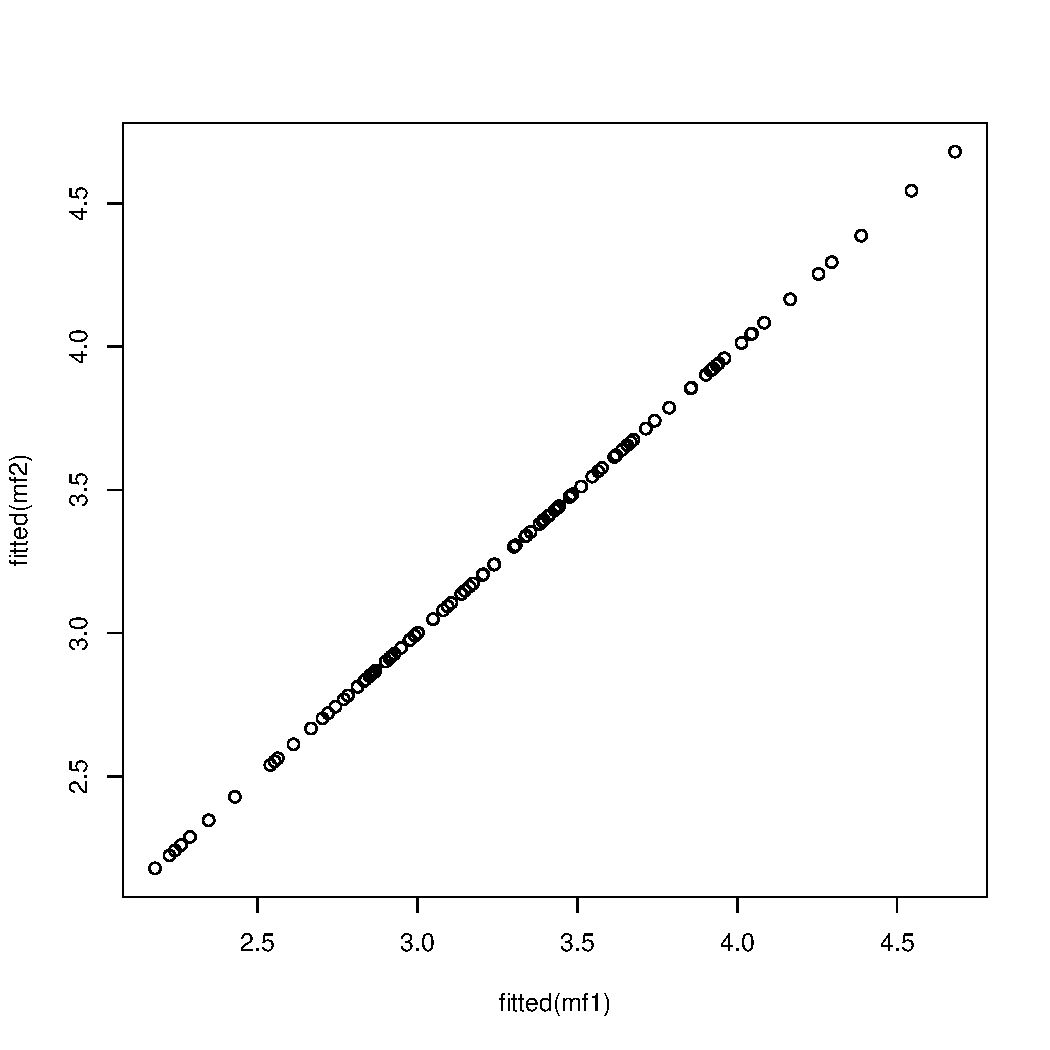
\includegraphics[width=\maxwidth]{figure/unnamed-chunk-13-1} 
\begin{kframe}\begin{alltt}
\hlkwd{plot}\hlstd{(}\hlkwd{resid}\hlstd{(mf1),} \hlkwd{resid}\hlstd{(mf2))}
\end{alltt}
\end{kframe}
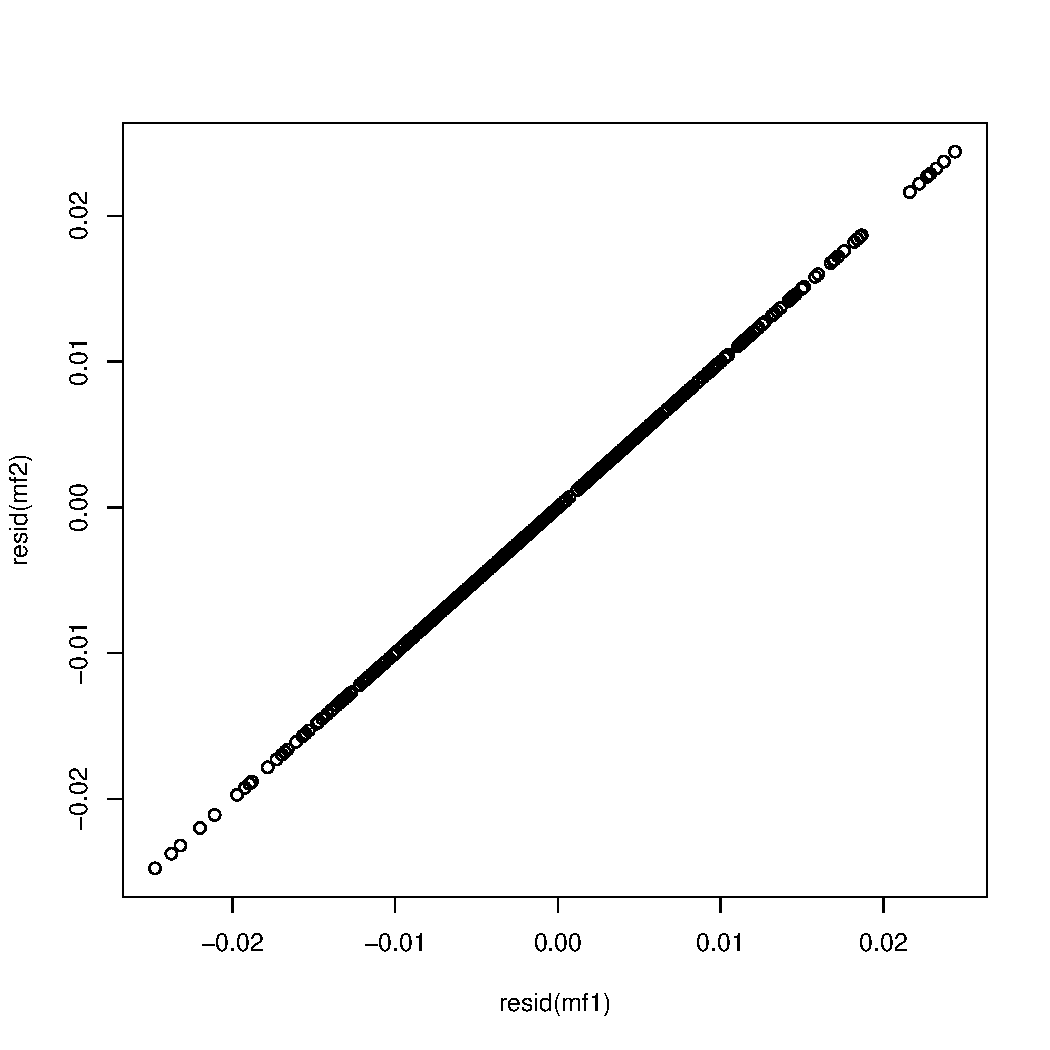
\includegraphics[width=\maxwidth]{figure/unnamed-chunk-13-2} 
\begin{kframe}\begin{alltt}
\hlkwd{AIC}\hlstd{(mf1)}
\end{alltt}
\begin{verbatim}
## [1] -2323
\end{verbatim}
\begin{alltt}
\hlkwd{AIC}\hlstd{(mf2)}
\end{alltt}
\begin{verbatim}
## [1] -2323
\end{verbatim}
\end{kframe}
\end{knitrout}
The two models are equivalent. Actually you can convert one into the other:

\begin{knitrout}
\definecolor{shadecolor}{rgb}{0.969, 0.969, 0.969}\color{fgcolor}\begin{kframe}
\begin{alltt}
\hlstd{vc1} \hlkwb{<-} \hlkwd{VarCorr}\hlstd{(mf1)}
\hlstd{vm1} \hlkwb{<-} \hlkwd{matrix}\hlstd{(vc1}\hlopt{$}\hlstd{id[}\hlnum{1}\hlopt{:}\hlnum{4}\hlstd{],} \hlkwc{nrow} \hlstd{=} \hlnum{2}\hlstd{)}

\hlstd{vc2} \hlkwb{<-} \hlkwd{VarCorr}\hlstd{(mf2)}
\hlstd{vm2} \hlkwb{<-} \hlkwd{matrix}\hlstd{(vc2}\hlopt{$}\hlstd{id[}\hlnum{1}\hlopt{:}\hlnum{4}\hlstd{],} \hlkwc{nrow} \hlstd{=} \hlnum{2}\hlstd{)}

\hlstd{trs} \hlkwb{<-} \hlkwd{matrix}\hlstd{(}\hlkwd{c}\hlstd{(}\hlnum{1}\hlstd{,}\hlnum{1}\hlstd{,} \hlnum{0}\hlstd{,}\hlnum{1}\hlstd{),} \hlkwc{nrow} \hlstd{=} \hlnum{2}\hlstd{)}

\hlstd{trs} \hlopt \hlstd{vm1} \hlopt \hlkwd{t}\hlstd{(trs)}
\end{alltt}
\begin{verbatim}
##        [,1]   [,2]
## [1,] 0.1740 0.2203
## [2,] 0.2203 0.3272
\end{verbatim}
\begin{alltt}
\hlstd{vm2}
\end{alltt}
\begin{verbatim}
##        [,1]   [,2]
## [1,] 0.1740 0.2203
## [2,] 0.2203 0.3272
\end{verbatim}
\end{kframe}
\end{knitrout}
\end{Answer}






\begin{Exercise}[difficulty=2, title={Beetles: build a model}]
Load the dataset "beetles.csv". It contains (fake) data from an (real) experiment on gene-by-environment interactions. The variable of interest is the mass of beetles born in two different environments, from different parents, and in different cages. Assuming that we can measure genetic varition with parent random effects, we wonder if different genomes respond differently to different environments.
\textbf{Build the model corresponding to this question in lme4.}

(hints: you could start from a lm() of mass modeled by environment, then add random intercepts, and finally a little something more).
\end{Exercise}

\begin{Exercise}[difficulty=2, title={Beetles: look at the model}]
What are the variances related to genetic differences? How are they correlated? Does genetic variation explain a lot of the total variation we observe? Try and draw a representation of genetic variation in the two environments. 
\end{Exercise}

\begin{Exercise}[difficulty=3, title={Beetles: interpret}]
Interpret model outputs (use raw numbers and / or graphes) to answer the following:
Is there evidence for genetic variation? Do the two environment differ in their effects on beetles? \\
Is there evidence for genetic variation in the response to the environment? \\
Does that mean that genomes good at environment 1 are bad at environment 2?
\end{Exercise}

\section{Correlated random effects}
In all of the above, we have assumed that random effect levels to be perfectly correlated (e.g., observations from the same year) or not at all correlated (e.g., observations from different years). It can be very interesting to allow for intermediate values, in particular for models of spatio-temporal autocorrelation, phylogenetics, quantitative genetics.


\subsection{Quantitative genetics}
Genes are transmitted from parents to offspring in a very predictable way: their genes have a correlation of 50\%. Therefore it is possible to estimate the genetic variance without any DNA sequencing when a dataset contains parents and offspring.
Going back to the long term monitoring of the wild animal population, let's load the population pedigree (ped.txt) and calculate this relatedness matrix:
\begin{knitrout}
\definecolor{shadecolor}{rgb}{0.969, 0.969, 0.969}\color{fgcolor}\begin{kframe}
\begin{alltt}
\hlkwd{library}\hlstd{(MCMCglmm)}
\end{alltt}


{\ttfamily\noindent\itshape\color{messagecolor}{\#\# Loading required package: coda}}

{\ttfamily\noindent\itshape\color{messagecolor}{\#\# Loading required package: ape}}\begin{alltt}
\hlstd{ped} \hlkwb{<-} \hlkwd{read.table}\hlstd{(}\hlstr{"ped.txt"}\hlstd{,} \hlkwc{header} \hlstd{=} \hlnum{TRUE}\hlstd{)}
\hlstd{ainv} \hlkwb{<-} \hlkwd{inverseA}\hlstd{(ped)}\hlopt{$}\hlstd{Ainv} \hlcom{#the inverse of relatedness matrix}
\hlkwd{image}\hlstd{(}\hlkwd{solve}\hlstd{(ainv)[}\hlnum{500}\hlopt{:}\hlnum{600}\hlstd{,}\hlnum{500}\hlopt{:}\hlnum{600}\hlstd{],} \hlkwc{useRaster}\hlstd{=T)} \hlcom{#the relatedness matrix}
\end{alltt}
\end{kframe}
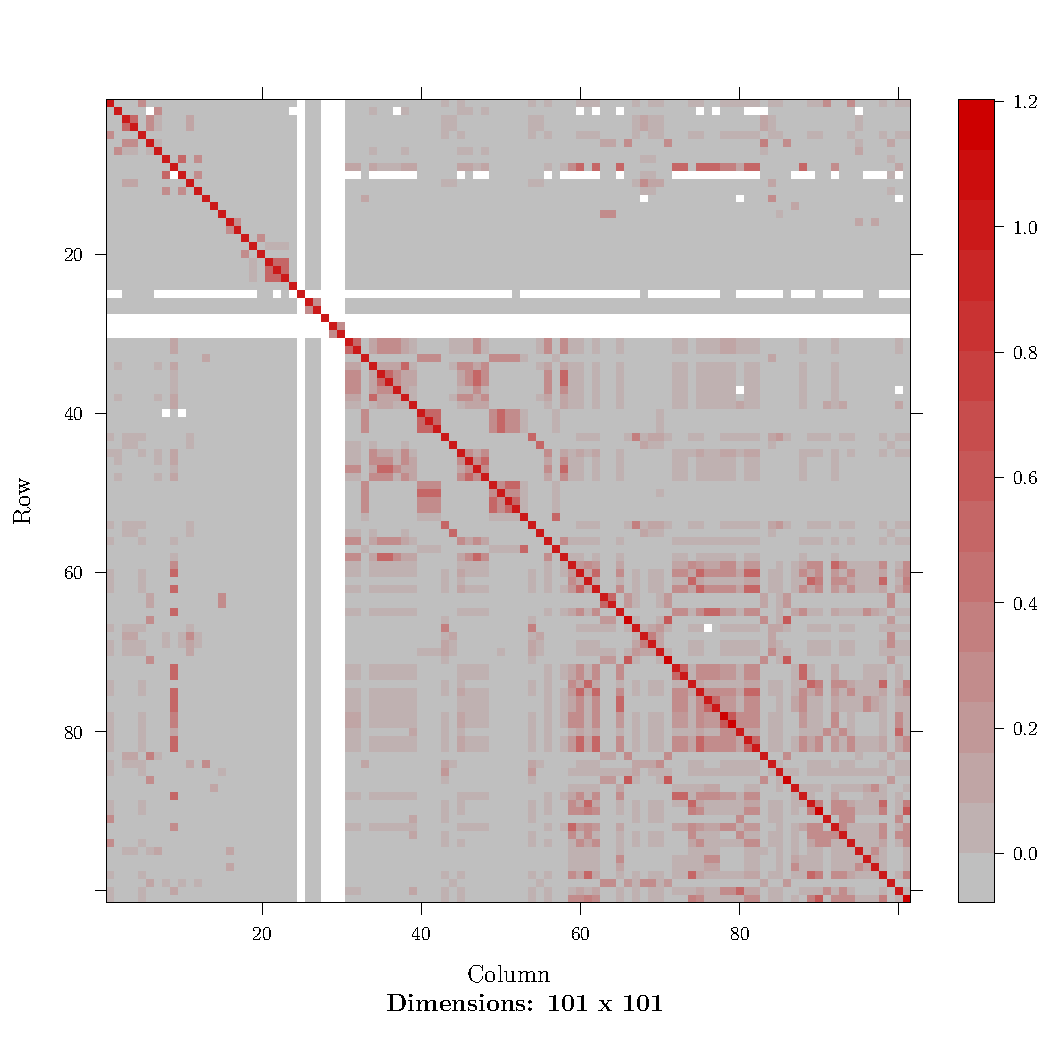
\includegraphics[width=\maxwidth]{figure/Gmatrix-1} 

\end{knitrout}

Is there genetic variation in weight? Here is a demonstration of fitting a quantitative genetic model.
\begin{knitrout}
\definecolor{shadecolor}{rgb}{0.969, 0.969, 0.969}\color{fgcolor}\begin{kframe}
\begin{alltt}
\hlstd{allm} \hlkwb{<-} \hlkwd{read.table}\hlstd{(}\hlstr{"AllM.txt"}\hlstd{,} \hlkwc{header} \hlstd{=} \hlnum{TRUE}\hlstd{)}

\hlstd{mweight} \hlkwb{<-} \hlkwd{MCMCglmm}\hlstd{(Weight} \hlopt{~} \hlnum{1} \hlopt{+} \hlstd{Age}\hlopt{*}\hlstd{Sex,} \hlkwc{random}\hlstd{=}\hlopt{~}\hlstd{Year} \hlopt{+} \hlstd{id,}
                    \hlkwc{ginverse} \hlstd{=} \hlkwd{list}\hlstd{(}\hlkwc{id}\hlstd{=ainv),} \hlkwc{data}\hlstd{=allm)}
\hlkwd{summary}\hlstd{(mweight)}
\end{alltt}
\end{kframe}
\end{knitrout}
The effect "id" has a large variance attached to it, suggesting the presence of a lot of genetic variation.

\begin{Exercise}[difficulty=1, title={Is it really genetic?}]
However that was a bit cheating, because individuals had several observations, so the "genetic" random effect may be just repeated measurements. Let's add another random effect for individual, but not connected to the relatedness matrix (you can use the variable "animal" which is a duplicate of "id"). 

\end{Exercise}
\begin{Answer}
\begin{knitrout}
\definecolor{shadecolor}{rgb}{0.969, 0.969, 0.969}\color{fgcolor}\begin{kframe}
\begin{alltt}
\hlstd{mweightG} \hlkwb{<-} \hlkwd{MCMCglmm}\hlstd{(Weight} \hlopt{~} \hlnum{1} \hlopt{+} \hlstd{Age}\hlopt{*}\hlstd{Sex,} \hlkwc{random}\hlstd{=}\hlopt{~}\hlstd{Year} \hlopt{+} \hlstd{id} \hlopt{+} \hlstd{animal,}
                     \hlkwc{ginverse} \hlstd{=} \hlkwd{list}\hlstd{(}\hlkwc{animal}\hlstd{=ainv),} \hlkwc{data}\hlstd{=allm,} \hlkwc{nitt} \hlstd{=} \hlnum{30000}\hlstd{)}
\hlkwd{summary}\hlstd{(mweightG)}
\end{alltt}
\end{kframe}
\end{knitrout}

\end{Answer}


\subsection{Phylogenetic model}

In a phylogenetic tree some species have a longer common evolutionary history than others. What those species look like may be influenced by the common evolutionary history. We can model that by considering phylogenetic correlations between two lineage as the time of common evolution relative to their outgroup. 


\begin{Exercise}[difficulty=1, title={Demo of Phylogeny and correlated phenotypes}]
Load a phylogeny of bird families and some bird phenoypes:
\begin{knitrout}
\definecolor{shadecolor}{rgb}{0.969, 0.969, 0.969}\color{fgcolor}\begin{kframe}
\begin{alltt}
\hlkwd{load}\hlstd{(}\hlstr{"birdfamilies"}\hlstd{)} \hlcom{#phylogeny. Loading creates the object bird.families}
\hlstd{birds} \hlkwb{<-} \hlkwd{read.csv}\hlstd{(}\hlstr{"birdpheno.csv"}\hlstd{)} \hlcom{#family phenotypes}
\end{alltt}
\end{kframe}
\end{knitrout}

To start, we subset the phylogeny to a few families
\begin{knitrout}
\definecolor{shadecolor}{rgb}{0.969, 0.969, 0.969}\color{fgcolor}\begin{kframe}
\begin{alltt}
\hlstd{bird.families} \hlkwb{<-} \hlkwd{makeNodeLabel}\hlstd{(bird.families)}
\hlstd{some.families} \hlkwb{<-} \hlkwd{c}\hlstd{(}\hlstr{"Certhiidae"}\hlstd{,} \hlstr{"Paridae"}\hlstd{,} \hlstr{"Gruidae"}\hlstd{,}
\hlstr{"Struthionidae"}\hlstd{)}
\hlstd{Nphylo} \hlkwb{<-} \hlkwd{drop.tip}\hlstd{(bird.families,} \hlkwd{setdiff}\hlstd{(bird.families}\hlopt{$}\hlstd{tip.label,}
\hlstd{some.families))}
\end{alltt}
\end{kframe}
\end{knitrout}
So we can easily visualize it:
\begin{knitrout}
\definecolor{shadecolor}{rgb}{0.969, 0.969, 0.969}\color{fgcolor}\begin{kframe}
\begin{alltt}
\hlkwd{plot}\hlstd{(Nphylo)}
\end{alltt}
\end{kframe}
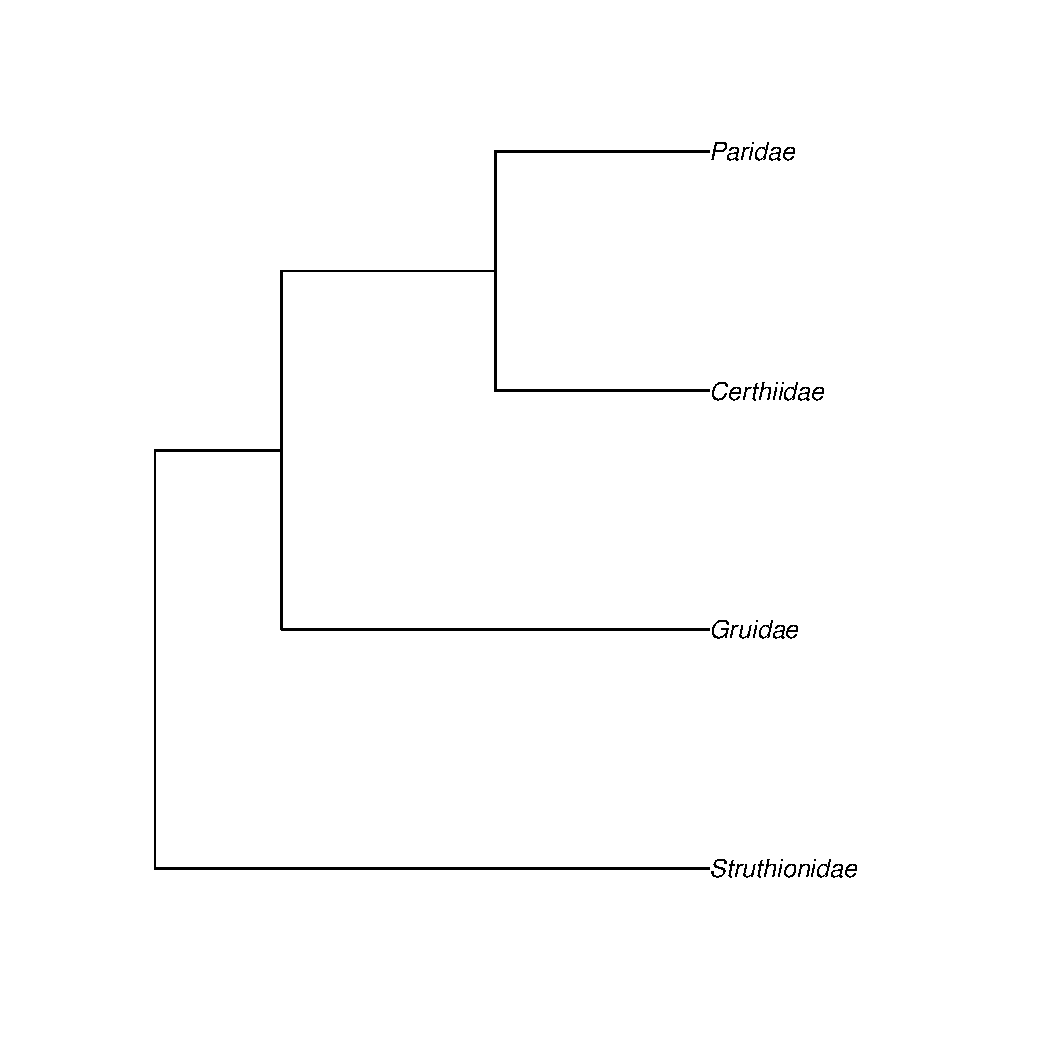
\includegraphics[width=\maxwidth]{figure/unnamed-chunk-20-1} 

\end{knitrout}
Which families will tend to have more similar phenotypes do you think?\\

We can calculate the variance covariance matrix of that tree as:
\begin{knitrout}
\definecolor{shadecolor}{rgb}{0.969, 0.969, 0.969}\color{fgcolor}\begin{kframe}
\begin{alltt}
\hlkwd{library}\hlstd{(MCMCglmm)}
\hlstd{INphylo} \hlkwb{<-} \hlkwd{inverseA}\hlstd{(Nphylo)}
\hlstd{sA} \hlkwb{<-} \hlkwd{as.matrix}\hlstd{(}\hlkwd{solve}\hlstd{(INphylo}\hlopt{$}\hlstd{Ainv))}
\hlkwd{colnames}\hlstd{(sA)} \hlkwb{<-} \hlkwd{rownames}\hlstd{(sA)} \hlkwb{<-} \hlkwd{rownames}\hlstd{(INphylo}\hlopt{$}\hlstd{Ainv)}
\hlstd{sA}
\end{alltt}
\begin{verbatim}
##               Node58 Node122 Struthionidae Gruidae Certhiidae Paridae
## Node58        0.2286  0.2286             0  0.2286     0.2286  0.2286
## Node122       0.2286  0.6143             0  0.2286     0.6143  0.6143
## Struthionidae 0.0000  0.0000             1  0.0000     0.0000  0.0000
## Gruidae       0.2286  0.2286             0  1.0000     0.2286  0.2286
## Certhiidae    0.2286  0.6143             0  0.2286     1.0000  0.6143
## Paridae       0.2286  0.6143             0  0.2286     0.6143  1.0000
\end{verbatim}
\end{kframe}
\end{knitrout}
What are the zero?\\

Coming back to the full dataset, we can fit a phylogenetic model as:
\begin{knitrout}
\definecolor{shadecolor}{rgb}{0.969, 0.969, 0.969}\color{fgcolor}\begin{kframe}
\begin{alltt}
\hlstd{INphylofull} \hlkwb{<-} \hlkwd{inverseA}\hlstd{(bird.families)} \hlcom{# Object contains inverse relatedness matrix, pedigree, inbreeding...}
\hlstd{prior0} \hlkwb{<-} \hlkwd{list}\hlstd{(}\hlkwc{G}\hlstd{=}\hlkwd{list}\hlstd{(}\hlkwc{G1}\hlstd{=}\hlkwd{list}\hlstd{(}\hlkwc{V}\hlstd{=}\hlnum{1}\hlstd{,} \hlkwc{nu}\hlstd{=}\hlnum{1}\hlstd{,} \hlkwc{alpha.mu}\hlstd{=}\hlnum{0}\hlstd{,} \hlkwc{alpha.V}\hlstd{=}\hlnum{100}\hlstd{)),}
               \hlkwc{R}\hlstd{=}\hlkwd{list}\hlstd{(}\hlkwc{V}\hlstd{=}\hlnum{1}\hlstd{,} \hlkwc{nu}\hlstd{=}\hlnum{0.002}\hlstd{))}
\hlstd{m1} \hlkwb{<-} \hlkwd{MCMCglmm}\hlstd{(y} \hlopt{~} \hlnum{1}\hlstd{,} \hlkwc{random} \hlstd{=} \hlopt{~}\hlstd{id,} \hlkwc{ginverse} \hlstd{=} \hlkwd{list}\hlstd{(}\hlkwc{id}\hlstd{=INphylofull}\hlopt{$}\hlstd{Ainv),}
               \hlkwc{data} \hlstd{= birds,} \hlkwc{prior} \hlstd{= prior0)}
\hlkwd{summary}\hlstd{(m1)}
\end{alltt}
\end{kframe}
\end{knitrout}
\end{Exercise}
\begin{Answer}

\end{Answer}

\end{document}
